\chapter{Risk-Free Assets}

\section{Time Value of Money}
$N\$$ after some time is way less than $N\$$ today, simply because of two main points that they are locked till future point and prices may increase due to inflation which will decrease the purchasing power. So one should be compensated for this postponed time. Usually, this compensation is said to be the interest.
\subsection{Simple Interest}
Suppose we deposit some amount into a bank to earn some interest. The future value is determined by initial deposit (Principal $P$), interest rate $r(>0)$ and time $t$. In case of simple interest, where our interest is not earning interest, the value of our investment at time $t \geq 0$ will be \begin{equation} V(t)=(1+rt)P \end{equation}
the number $1+rt$ is called the growth factor.
If the Principal is invested at time $s$, then the value at time $t(\geq s)$ will be \begin{equation} V(t)=(1+r(t-s))P \end{equation}

\begin{figure}[htp]
    \centering
    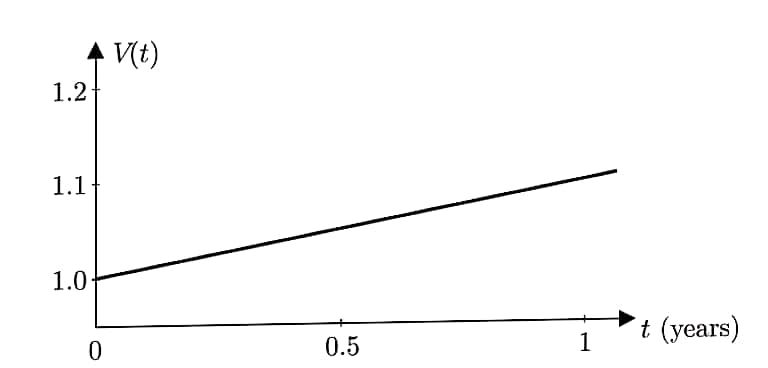
\includegraphics[width=15cm]{1.jpg}
    \caption{Principal attracting simple interest at 10\% $(r=0.1,P=1)$}
    \label{fig:SI}
\end{figure}

The return of this investment will be \begin{equation} K(s,t)=\frac{V(t)-V(s)}{V(s)} \end{equation}

In case of simple interest, \begin{equation} K(s,t)=r(t-s) \end{equation}
It is clear that interest rate is equal to return over one year (put $t=s+1$ in equation 2.4).
\\Present/discounted value of $V(t)$ is given by
\begin{equation}V(0)=V(t)(1+rt)^{-1}.\end{equation}
where $(1+rt)^{-1}$ is called the discount factor.
\paragraph{A perpetuity is a sequence of payment of fixed amount to be made at equal time intervals and continuing indefinitely into the future (e.g. -  Rent on real estate). For example, an initial deposit of $\frac{P}{r}$ will get you $P$ amount payable every year (in case of simple interest).}
\subsection{Periodic Compounding}
Generally simple interest is used only for short term investments or some specific loans. In principal, your earned interest also earns interest periodically, which is known as \textbf{compounding}. If $m$ interest payments are made per annum and the interest rate $r$ remains unchanged, after $t$ years the future value of an initial principal $P$ will become
\begin{equation}
    V(t)=(1+\frac{r}{m})^{tm} P
\end{equation}
where $t$ must be a whole multiple of $\frac{1}{m}$. The number $(1+\frac{r}{m})^{tm}$ is the growth factor.

\begin{figure}[htp]
    \centering
    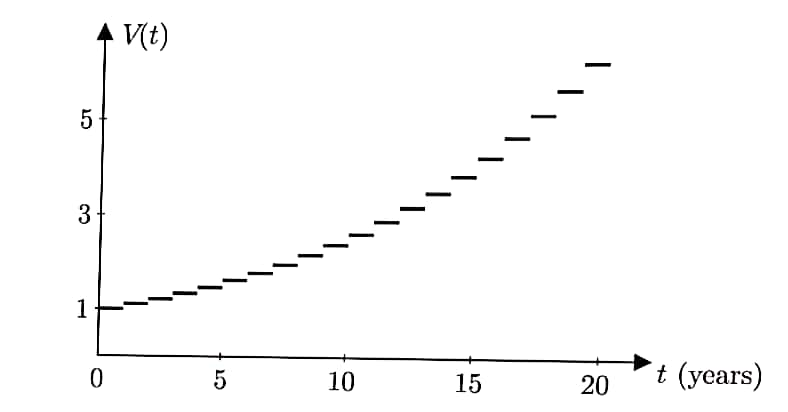
\includegraphics[width=10cm]{2.jpg}
    \caption{Annual compounding at 10\% $(m=1,r=0.1,P=1)$ }
    \label{fig:CI}
\end{figure}
%\vspace{10mm}
The return of this investment will be 
\begin{equation} 
K(s,t)=\frac{V(t)-V(s)}{V(s)}=(1+\frac{r}{m})^{(t-s)m}-1 
\end{equation}
It is clear that interest rate is equal to return over one year provided $m=1$ (put $t=s+1$ in equation 2.7).
\\Clearly, the return $K(s,t)$ is not additive $\{\because K(0,1)+K(1,2)\neq K(0,2)\}$
\\In case of compound interest, the present/discounted value of $V(t)$ is
\begin{equation}
    V(0)=V(t) (1+\frac{r}{m})^{-tm},
\end{equation}
where the number $(1+\frac{r}{m})^{-tm}$ is the discount factor.
\paragraph{It can be proven easily (using binomial formula) that the future value $V(t)$ increases if $m,t,r$ or $P$ increases. Also if $V(t)$ is kept fixed, present value increases if $r,t$ or $m$ decreases.}

\subsection{Streams of Payments}
\paragraph{An annuity is a sequence of finitely many payments of a fixed amount due at equal time intervals (e.g. - Regular Deposit to a savings account). For example, regular deposit of $P$ (with annual compound interest $r$) made once a year for n years will have the present value \-
\[\begin{split}
        PV=\frac{P}{1+r}+\frac{P}{(1+r)^{2}}+\cdots+\frac{P}{(1+r)^{n}}
        = P \times \frac{1-(1+r)^{-n}}{r}
        = P \times PA(r,n)
\end{split}\]
where $PA(r,n)$ is called present value factor for an annuity.
\\Formula for present value of a perpetuity can be obtained from above equation by letting $n\to\infty$ 
\[\displaystyle \lim_{n\to\infty} P \times PA(r,n) = \frac{P}{r}\]
We can observe that this is the same value as we studied in the case of simple interest. The reason is that the amount remaining to earn interest in the following year is always $\frac{P}{r}$. 
}
\subsection{Continuous Compounding}
Suppose the invested money is compounded annually and one withdraws the money after $11$ months, the person gets no interest. If $m \to \infty$ in equation (2.6), we get
\begin{equation}
    V(t)=e^{tr}P
\end{equation}
which is called continuous compounding. The growth factor is $e^{tr}$. The rate of growth is directly proportional to the current wealth. It gives higher returns compared to any frequency $m$.
In case of continuous compounding, the present/discounted value of $V(t)$ is
\begin{equation}
    V(0)=V(t) e^{-tr},
\end{equation}
where the number $e^{-tr}$ is the discount factor.

\begin{figure}[htp]
    \centering
    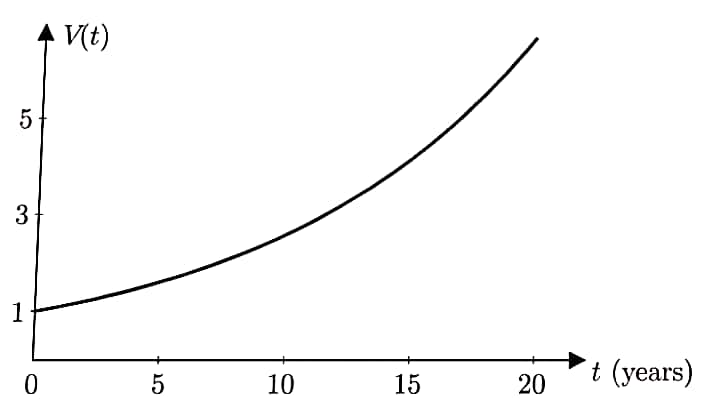
\includegraphics[width=15cm]{3.jpg}
    \caption{Continuous compounding at 10\% $(r=0.1,P=1)$}
    \label{fig:CC}
\end{figure}

Clearly, the usual return $K(s,t)$ is not additive $\{\because K(0,1)+K(1,2)\neq K(0,2)\}$, so we introduce the logarithmic returns \-
\begin{equation} 
k(s,t)=\ln \frac{V(t)}{V(s)} = (t-r)s.
\end{equation}
Note that, logarithmic returns are additive. $\{k(s,t)+k(t,u)=k(s,u)\}$
\subsection{How to Compare Compounding Methods}
We say that two compounding methods are equivalent if the corresponding growth factors over a period of one year are the same. If first growth factor exceeds the second, we say that the first method is preferable. For example, 10\% semi-annual compounding (growth factor = $(1+\frac{0.1}{2})^{2} =1.1025$) is preferable to 9\% monthly compounding (growth factor = $(1+\frac{0.9}{12})^{12} =1.0938$).
\\For a given compounding method with interest rate $r$ the effective rate $r_{e}$ is one that gives the same growth factor over the one year period under annual compounding, i.e. -

$1+r_{e}= \left\{ 
  \begin{array}{ c l }
    (1+\frac{r}{m})^{m} & \quad \textrm{, Periodic compounding}\\
    e^{r}                 & \quad \textrm{, Continuous compounding}
  \end{array}
\right.$
\\Hence two compounding methods are equivalent if and only if the corresponding effective rates are equal. If first effective rate exceeds the second, we say that the first method is preferable.
\\In terms of the effective rate $r_{e}$ the future value can be written as \begin{equation}
    V(t)=(1+r_{e})^{t}P, \hspace{10mm} \forall t \geq 0.
\end{equation}
\subsubsection{Cash flows of several payments}
Consider a time interval $[0,T]$ divided into $m$ equal sub-intervals, say $(t_{i},t_{i+1})$, with r interest rate per sub-interval, $t_{0}=0$ and $t_{m}=T$. We invest $P_{i} (\in \mathbb{R})$ after the end of $i^{th}$ sub-interval $(\forall i \geq 0)$. Negative $P_{i}$ shows the amount invested and positive $P_{i}$ shows the amount withdrawn. The future value of these cash flows\\
$V(T)= \left\{ 
  \begin{array}{ c l }
    \displaystyle \sum_{i=0}^{m} P_{i}(1+r)^{(m-i)} & \quad \textrm{, Periodic compounding}\\
    \displaystyle \sum_{i=0}^{m} P_{i}e^{r(T-t_{i})}                 & \quad \textrm{, Continuous compounding}
  \end{array}
\right.$
\\Suppose we need to compare two project with complex investments and pick out the better one.  The investment with better present value will be the better one.The present value of these cash flows\\
$V(0)= \left\{ 
  \begin{array}{ c l }
    \displaystyle \sum_{i=0}^{m} \frac{P_{i}}{(1+r)^{i}} & \quad \textrm{, Periodic compounding}\\
    \displaystyle \sum_{i=0}^{m} \frac{P_{i}}{e^{rt_{i}}}                 & \quad \textrm{, Continuous compounding}
  \end{array}
\right.$